\documentclass[addpoints,11pt]{exam}

\usepackage[margin=2.5cm]{geometry}
\usepackage{graphicx}
\usepackage{listings}
\usepackage{xpatch}
\usepackage{color}
\usepackage{amsmath}
\usepackage{hyperref}

\makeatletter
\xpretocmd{\item@points@pageinfo}{\normalfont}{}{}
\xapptocmd{\item@points@pageinfo}{\bfseries}{}{}
\makeatother

\begin{document}
	\begin{center}
		\LARGE\scshape{Structure-dependent behaviours of skin layers studied by atomic force microscopy}
		\vspace{0.5cm}
		
		\large DOI: 10.1111/jmi.12562
		
		\vspace{1cm}
		\large\scshape{Juan Barbosa - 201325901}
	\end{center}
	
	La multicapa de la piel es de mayor importancia en los mam\'iferos, dado que provee de resistencia f\'isica y protege del medio ambiente. Actualmente la microscop\'ia \'optica es la t\'ecnica m\'as usada en la investigaci\'on de los tejidos de piel, sin embargo es posible obtener la misma informaci\'on junto con otra adicional usando microscop\'ia de fuerza at\'omica (AFM). Lo anterior es posible dado que existe una diferencia en la resistencia mec\'anica en los constituyentes del tejido y sus fronteras, lo cual permite su cuantificaci\'on y caracterizaci\'on por AFM.
	
	Los dos m\'etodos m\'as usados para la caracterizaci\'on de la piel son: tomograf\'ia de coherencia \'optica, la cual permite ver hasta 3 mm de profundidad en la muestra; y la tinción con hematoxilina-eosina. Ambas t\'ecnicas presentan resoluci\'on de micr\'ometros. Es ac\'a donde AFM tiene una ventaja importante, puesto que por un lado mejora la resoluci\'on hasta la escala nano, obteniendo im\'agenes de alta resoluci\'on, adem\'as de detectar las propiedades mec\'anicas de la muestra.
	
	El experimento se llev\'o a cabo usando ratones de 8 semanas \textit{C57Bl/6JNarl}, a los cuales luego de haberseles anestesiado recibieron quemaduras con laser de longitudes entre 3 mm y 20 mm, posteriormente se estudiaron esp\'ecimes con un tiempo de curado de 3 y 7 d\'ias. Los estudios microsc\'opicos se llevaron a cabo usando disecciones de 3 $\mu$m de grosor. En el AFM se usaron como par\'ametros una frecuencia de escaneo de 0.3 Hz y 512 pixeles, junto con una punta de nitruro de silicio con constante de 0.7 N m$^{-1}$.
	
	La figura siguiente muestra los resultados en t\'erminos de resoluci\'on, donde todas las im\'agenes de AFM (derecha) est\'an incluidas en el campo de visi\'on de la t\'ecnica \'optica (izquierda).
	\begin{figure}[h]
		\centering
		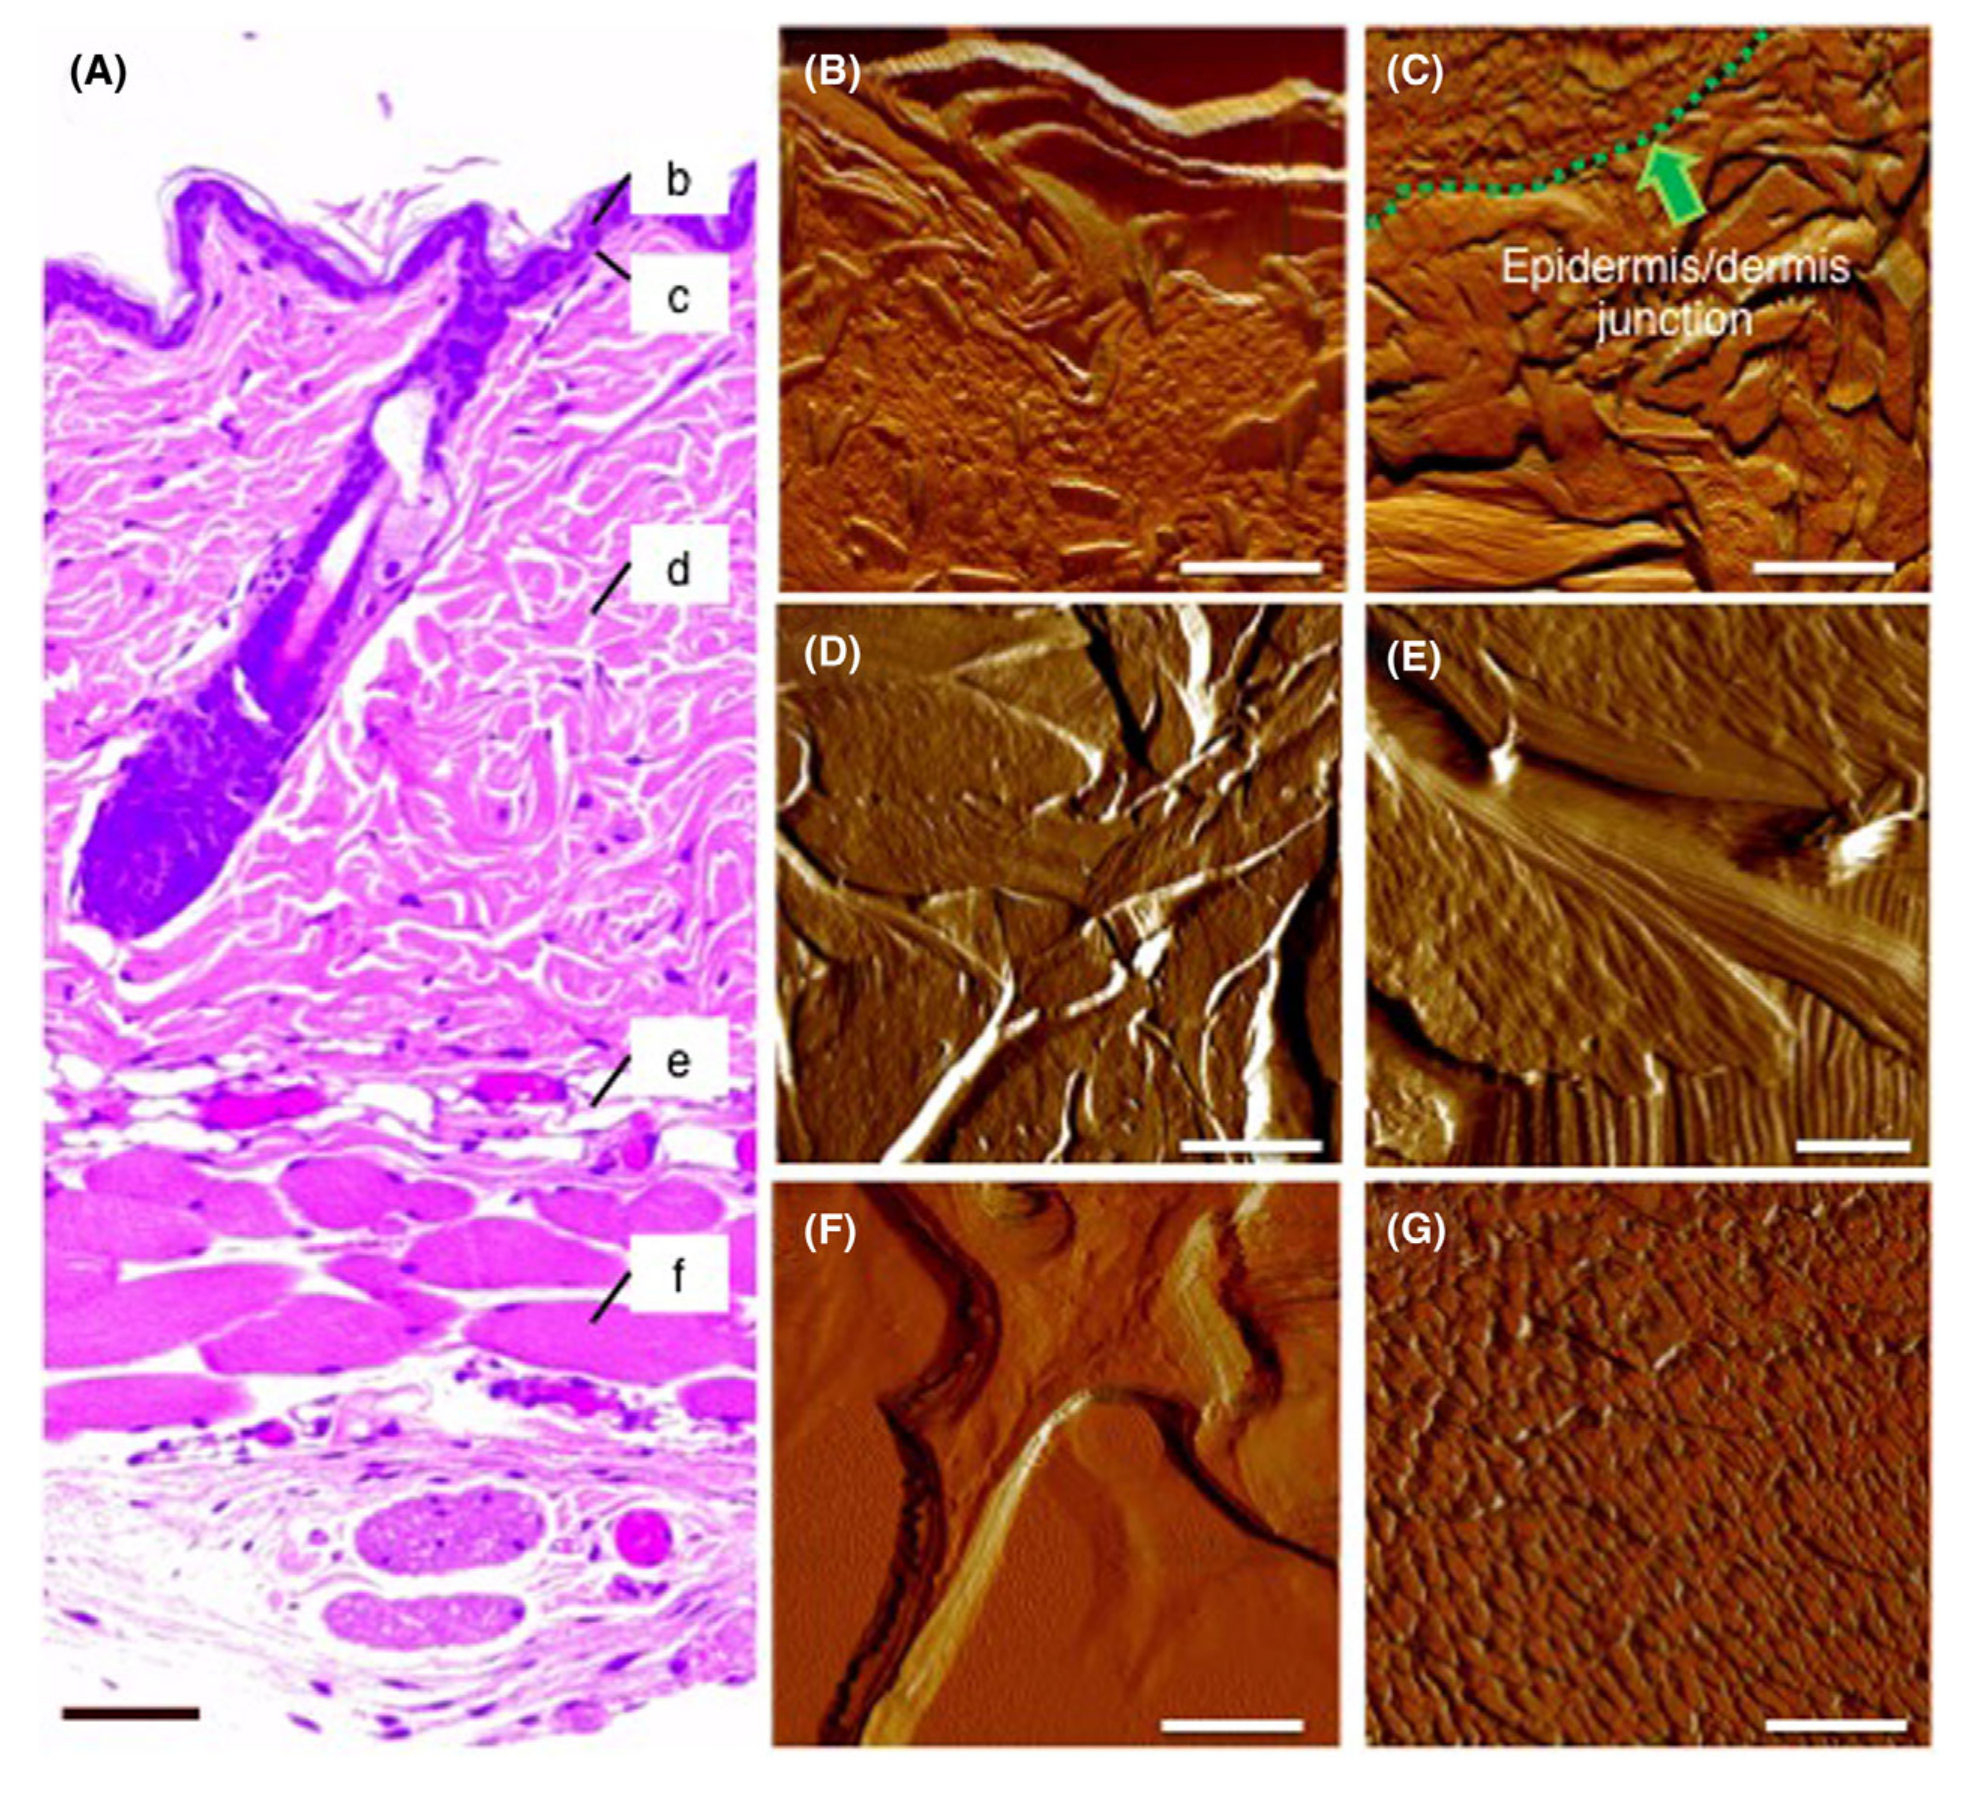
\includegraphics[width=0.6\linewidth]{chang2017.png}
	\end{figure}
	\newpage
	
	En particular en la figura (D), se observ\'o una gran cantidad de fibras de col\'ageno, las cuales se atribuyen a la funci\'on de protecci\'on del cuerpo al estr\'es externo, juntando el epidermis con las capas subcut\'aneas. Un an\'alisis de tomograf\'ia 3D permiti\'o observar las diferencias entre la piel con curaci\'on de 3 d\'ias junto con la de 7. La mayor diferencia fue la cantidad de c\'elulas inflamatorias en la muestra, por lo cual se concluye que dentro de los 3 d\'ias la piel se encuentra en la etapa de inflamaci\'on. A los 7 d\'ias se encuentra una etapa entre inflamaci\'on y re-epitalizaci\'on, esto debido a la presencia de col\'ageno del tipo III.
\end{document}